\textit{Sections to be incorperated into other parts of the report}

% Compression Performance Metrics
\subsubsection{Chrominance Downsampling}

JPEG leverages a YCbCr colorspace in order to distinguish between Luminance and Chrominance information in the image.
This distinction allows for the Chrominance Channels to be downsampled while the Luminance stays full rank.
In this section we analyze the effects of downsampling on our compressed image quality metrics. 
Shown in figure \ref{fig:downsample_vs_psnr}, downsampling uniformly reduces PSNR and compression rate. However, unlike Quantization, image quality drops off steeply and compression rate does not improve significatly for large downsample factors.

\begin{figure}
    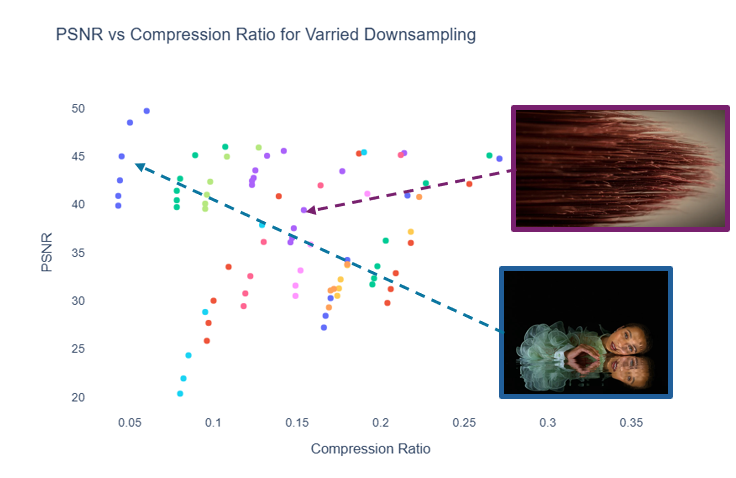
\includegraphics[width=0.5\textwidth]{assets/PSNR vs Chromiance Downsampling with Images.png}
    \caption{As expected, generally increasing the chromiance downsample rate (and therefore reducing the compression ratio), the PSRN metric is degraded.}
    \label{fig:downsample_vs_psnr}
\end{figure}

\subsubsection{Block Size}

For this experiment we vary the block size according to table \ref{tab:Block Size Sweep}. We find the larger blocks do not compress the images as much as small blocks \ref{fig:block_comp_rates}. Additionally, varrying the block size also does not see to effect the PSNR to a large extent. However, qualitatively the blocking strategies are visibly different \ref{fig:block_quantization_artifacts}. The effect of smaller blocks is that the edges of each block becomes more clearly visible, giving the effect that the entire image has been downsampled in 2x2 pixel blocks. In larger blocks, there are shimmers and other quantization artifacts which are visible across the block upon close inspection, despite the block edges being less obvious. It's clear that a small block with a reasonable compression rate, that preserves a gradient over the block while minimizing frequency quantization artifacts is ideal for image visual appeal.

\begin{figure}
    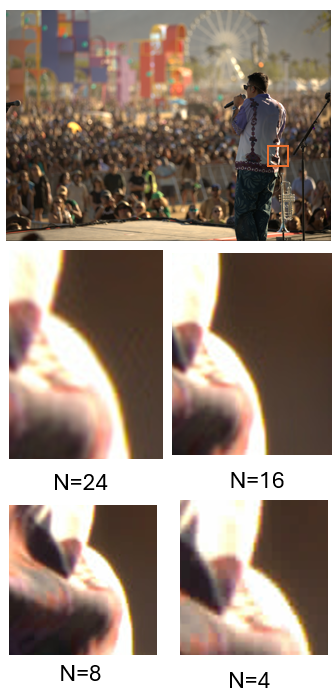
\includegraphics[width=0.5\textwidth]{assets/Block Quantization Artifacts.png}
    \caption{A visualization of block size artifacts. As blocks become larger, individual blocks have more detail, and features within the blocks are more clear, but block boundaries are still visible.}
    \label{fig:block_quantization_artifacts}
\end{figure}

\begin{figure}
    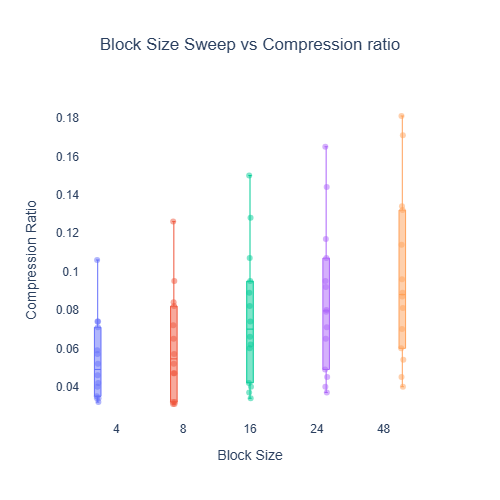
\includegraphics[width=0.5\textwidth]{assets/Comp Rate VS block Size.png}
    \caption{Compression Rates improve with smaller block sizes, while larger block sizes result in overall larger image size, despite the same relative quantization being applied across block sizes.}
    \label{fig:block_comp_rates}
\end{figure}

\begin{figure}
    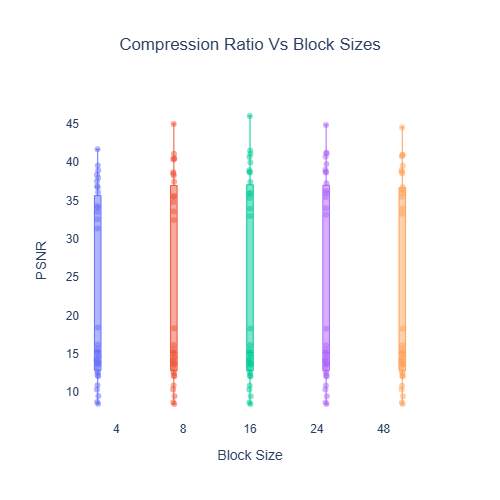
\includegraphics[width=0.5\textwidth]{assets/Block Size Vs PSNR.png}
    \caption{As block size is varried with quantization kept relativly the same, the PSNR does not change.}
\end{figure}

\subsection{Runtime and Performance}

One main difference between our compression pipeline JPEG compression is that the huffman tables are not pre-computed. Through our tests we note that this accounts for a significant portion of the computational load for compression and decompression \ref{fig:runtimes}. It is important to note that these runtimes are not comparable to well established codex standards, as most machines have dedicated hardware for performing these computations. The computed runtimes are only comparable to other internal results. 

\begin{figure}
    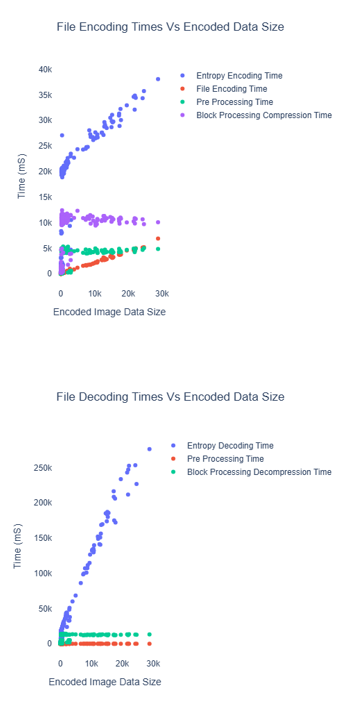
\includegraphics[options]{assets/Runtimes Summary.png}
    \caption{Sets of sampled runtimes for the most computationally intensive parts of the our flexible compressoin pipeline.}
    \label{fig:runtimes}
\end{figure}